\section{System Architecture} \label{sec:sysarc}


The LSST control system is based on a reactive data-driven actor-based architecture that uses a multi cast Data Distribution Service (DDS) messaging protocol middleware. A high level view of this architecture is given in \figref{fig:arc}, where each box corresponds to a component of the system (not all components are displayed here). 

The LSST System Architecture is comprised mainly of;
%
\begin{itemize}
\item The Service Abstraction Layer (SAL\footnote{\url{https://docushare.lsstcorp.org/docushare/dsweb/Get/Document-21527/}}) communication middleware. Based on the DDS protocol, it provides interfaces for all the project adopted programming languages (LabView, C++, Java and Python).
\item Engineering and Facility Database (EFD).
\item SAL-aware reactive components, a.k.a Commandable SAL Components (CSCs). 
\item LSST Operators Visualization Environment (LOVE).
% \item Python SalObj\footnote{\url{https://github.com/lsst-ts/ts_salobj}} library.
%\item LabView component template. 
% \item Script Queue  \footnote{\url{https://github.com/lsst-ts/ts_scriptqueue}}
\end{itemize}

\begin{figure}
\begin{center}
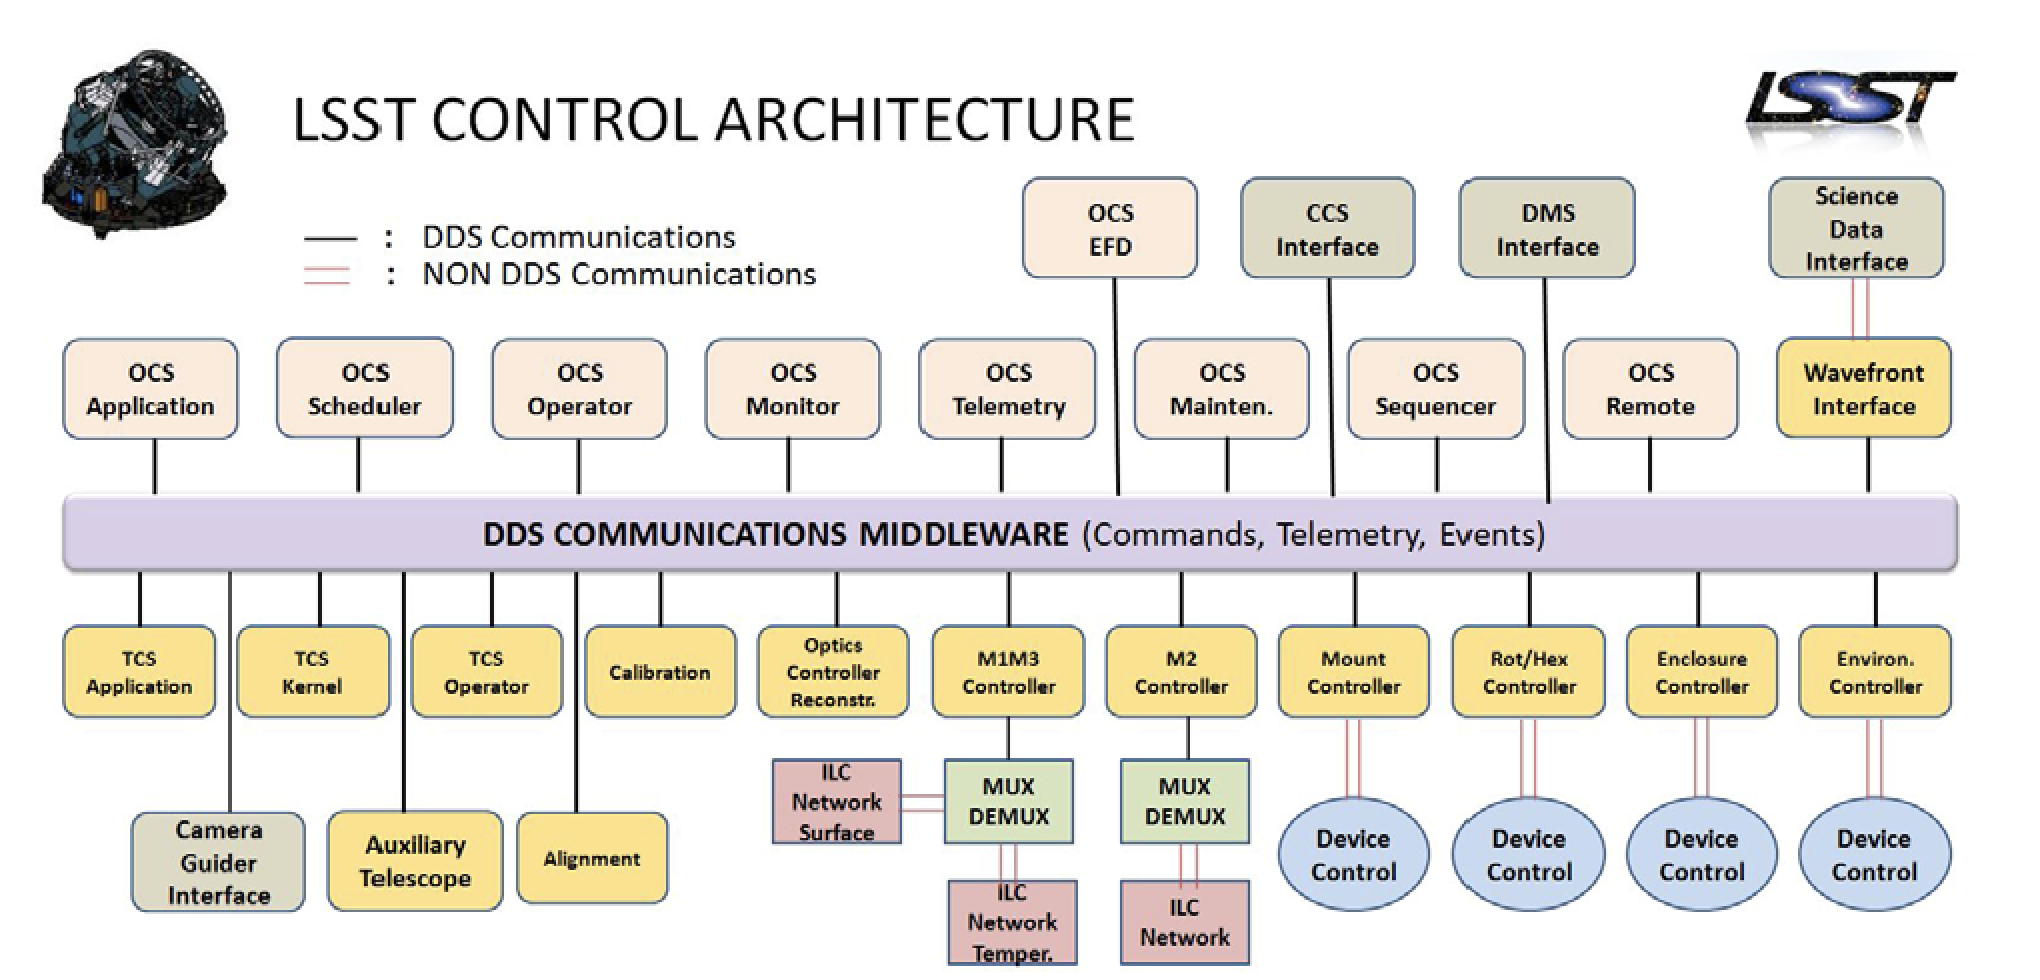
\includegraphics[width=0.8\textwidth]{arc}
\caption{High Level Architecture Diagram\label{fig:arc}}
\end{center}
\end{figure}

The SAL middleware is the backbone of the LSST system architecture. It implements three distinct types of messages; Commands, Events and Telemetry, with distinct purposes. Commands are sent to a specific component, which must acknowledge its receipt and perform some action. In general, the receiving component will be the only entity listening for the commands it accepts. Events and Telemetry are messages broadcasted by components to the middleware and are available to any entity on the system to receive. The distinction between Events and Telemetry is that the former receives a higher priority by the message passing systems. 

The EFD is responsible for capturing all SAL messages broadcasted to the middleware (including Commands, Events and Telemetry) and storing that information into a database. 

CSCs are the main actors of the LSST system architecture. They are responsible for managing the incoming traffic of data and take appropriate actions, controlling hardware (e.g. M1M3, M2, Mount Controller, etc in Fig.~\ref{fig:arc}), software (e.g. Optics Controller Reconstructor, DMCS Interface, etc in Fig.~\ref{fig:arc}) or even other CSCs (e.g. Script Queue, TCS, ATCS, OCS, etc in Fig.~\ref{fig:arc} ).

LOVE is responsible for capturing SAL messages and displaying them in a useful way for general users, providing some basic interface to query and analyze data from the EFD and an interface to issue some pre-defined commands to a set of components.

One of the fundamental parts of SAL is to provide a low-level API for publishing and subscribing to the middleware. These APIs are generated for each component independently, based on pre-defined interfaces. On top of those low level APIs, developers have access two higher level set of frameworks; Python SalObj\footnote{\url{https://github.com/lsst-ts/ts_salobj}} library and the LabView component template. No higher level framework is supported for implementation in Java or C++. 

% a Python library (e.g. SalObj) or the LabView component template. There is no higher level support for implementation in Java or C++. 

% Each component of the system is and independent actor that reacts to data published to the middleware. 

%\begin{itemize}
%\item Infrastructure and Middleware :
%\item The Scheduler \footnote{\url{https://github.com/lsst-ts/ts_scheduler}}
%\item Potentially an Auxiliary and Main Telescope Control System (ATCS and TCS)\footnote {The precise nature and need for these is unclear now so they have lower priority.}
%\item Controllable SAL Components (CSCs) - every device and some pseudo devices, including the scheduler, are CSCs. Some are coordinating other CSCs, the full hierarchy is shown for AuxTel in \figref{fig:atcscs} and the Main Telescope in \figref{fig:mtcscs}
%\end{itemize}

Overall, the system architecture can be divided into three main namespaces; Observatory, Main Telescope (MT) and Auxiliary Telescope (AT). The Observatory is the highest level and encapsulates both the Main Telescope, Auxiliary Telescope and global components such as the weather station, DIMM, etc. The complete set of components that belong to each of these namespaces can be seen in Figs.~\ref{fig:ocs}, ~\ref{fig:atcscs} and \ref{fig:mtcscs}.

\begin{figure}
\begin{center}
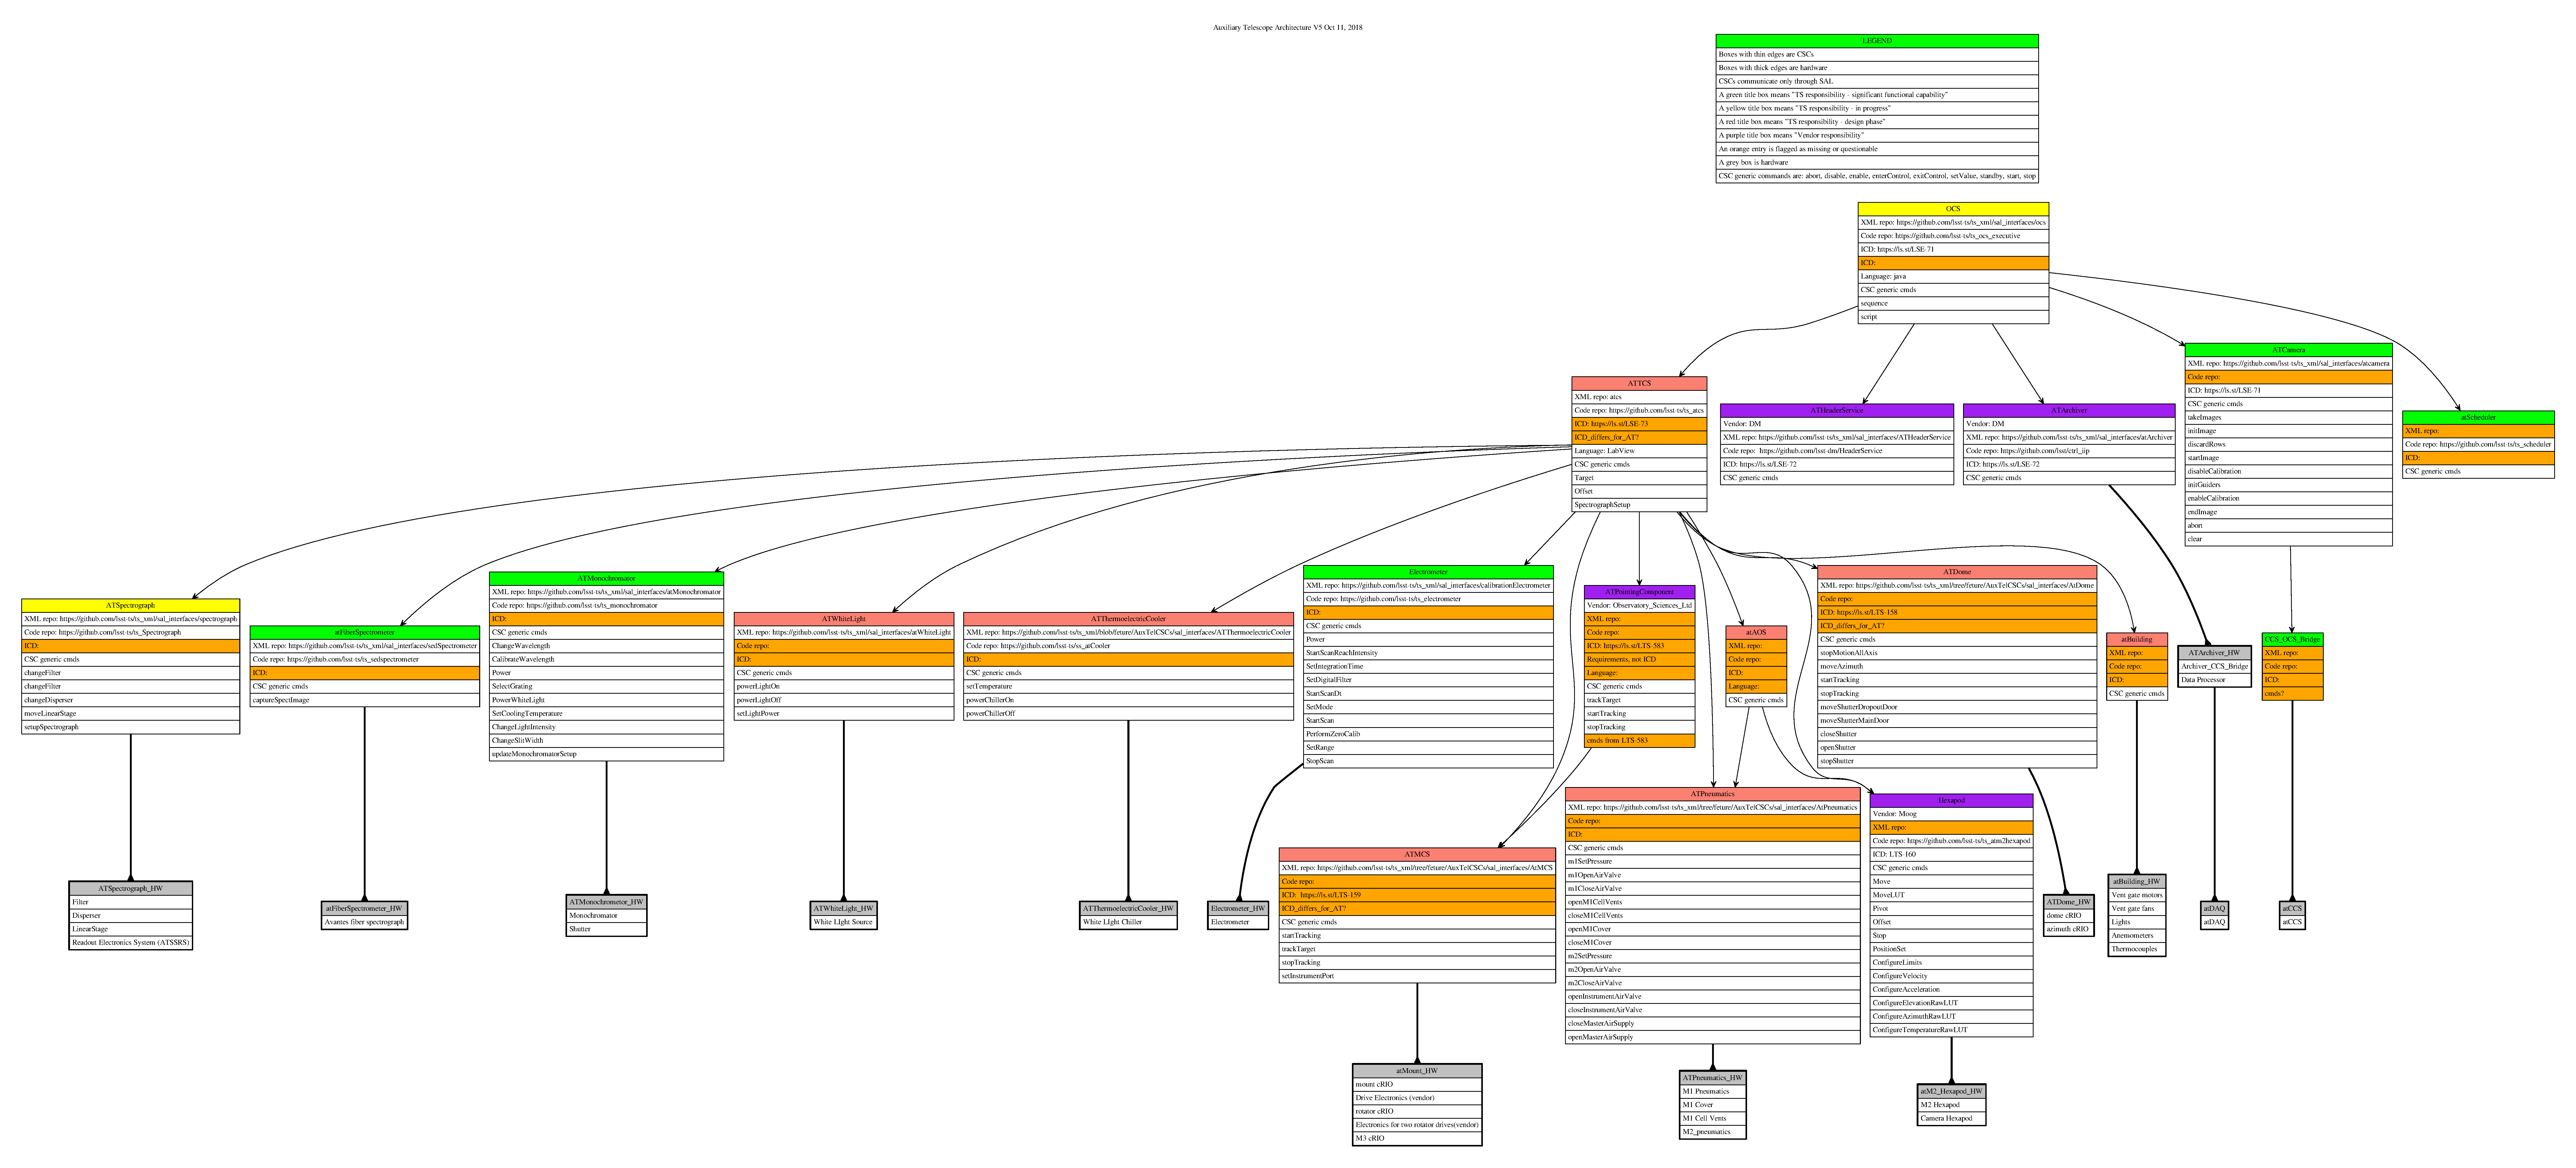
\includegraphics[width=0.9\textwidth]{AT}
\caption{Complete set of AT CSCs\label{fig:atcscs}}
\end{center}
\end{figure}

\begin{figure}
\begin{center}
\includegraphics[width=0.9\textwidth]{LSST}
\caption{Complete set of MT CSCs\label{fig:mtcscs}}
\end{center}
\end{figure}

\subsection{SalObj - Python and scripting }\label{sect:salobj}
SalObj is a Python library provides a pythonic and object-oriented interface to create CSCs and Scripts that can be executed by the script queue component (see Sect.~\ref{sect:scriptq}). The library defines two sets of base classes that are mirror to each other, Remote and Controller. A Remote will send commands to and receive telemetry and events from a specific component whereas a Controller will receive commands and publish telemetry and events. In this framework, a CSC is a specialized Controller that is configure to perform some basic actions by default. A high level diagram is provided in \figref{fig:salobj}.

Internally, SalObj uses the python library \asyncio\footnote{\url{https://docs.python.org/3/library/asyncio.html}} to handle the inherently asynchronous nature of the SAL messaging system. 

\begin{figure}
\begin{center}
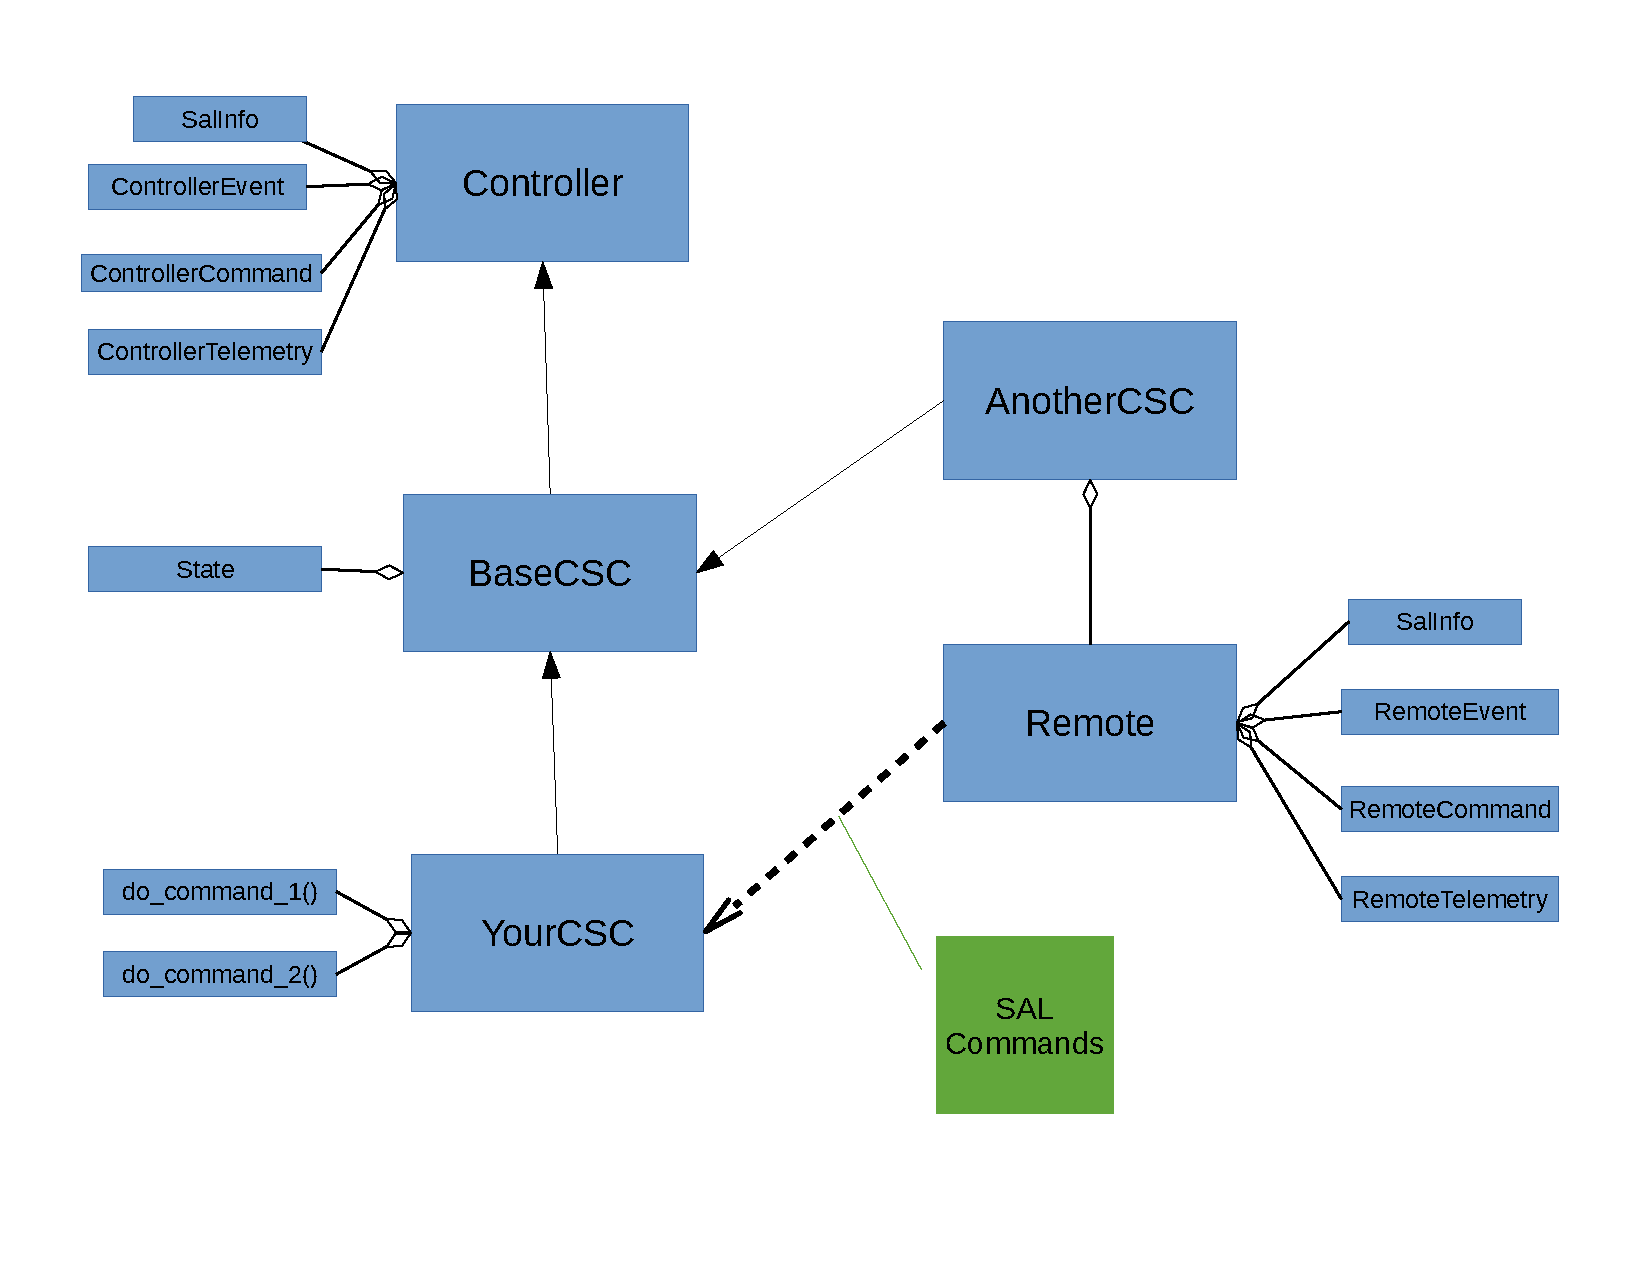
\includegraphics[width=0.9\textwidth]{SalobjClassDiag2}
\caption{SalObj python scheme for  CSCs\label{fig:salobj}}
\end{center}
\end{figure}

\subsection{Hardware interface components}\label{sect:hardware_csc}
Probably the most critical or sensitive components of the LSST system architecture are those that directly control hardware. Some of these components are going to be delivered directly by external vendors, such as those that will control the main telescope mount (MTMount) and the main telescope secondary mirror (MTM2). There are also those that are developed in house, e.g. the main telescope M1M3 (MTM1M3). 

In some special cases it is highly desirable that the control software and hardware are part of an integrated system. For those systems, the components are developed either using the LabView component template, which is part of the LSST infrastructure or in C++ developed using the low level SAL API. 

On most other cases, the hardware comes with a control software that can be easily interfaced by using broadly used standard protocols (such as TCP/IP or serial ports), and there is no special need for the component software to reside close to the low level hardware controller. In those cases, the components are written in Python using the SalObj library which is also part of the LSST infrastructure. By writing these components in Python we allow a high level of flexibility and maintainability of the software components and considerably decrease the development cycle. 

\subsection{Pure software components}\label{sect:software_csc}
In the LSST System Architecture there are a number of components that, even tough they do not control hardware directly, they dictate what hardware components are supposed to do. Some of these components are responsible for heavy computational routines, such as the Optical Feedback Control (MTOFC), which is responsible for applying corrections to both M1M3, M2 and hexapod components for the main telescope or even the Scheduler, which is responsible for processing the an entire set of observatory telemetry information and history of observations to compute an observing queue. 

These pure software components are mostly written in Python using SalObj library. There are three special cases of these components that form the basis of the LSST System Architecture; the Script Queue (Sect.~\ref{sect:scriptq}), Control Systems (Sect.~\ref{sect:ocs}) and the Watcher (Sect.~\ref{sect:watcher}). Together, they provide the tools needed for integration, commissioning and operation of the observatory.  

\subsubsection{The ScriptQueue component} \label{sect:scriptq}
There are a number of different ways users can interact with components in the LSST system. For instance, one could easily use the SAL generated API in any of the supported languages to send commands directly to a single or multiple components. It is also possible to use SalObj Remotes to write Python scripts that would command different components to accomplish a specified task. Not to mention that LOVE itself provides a customizable interface for users to interact with components. 

During commissioning and operations the LSST system will require a high degree of coordination between different crews (different daytime and nighttime shifts, for instance), not to mention the increasing number of available components and level of complexity as the system ramps up. In order to manager those issues, the LSST control system contains a specialized script queueing component, a.k.a. the ScriptQueue\footnote{\url{https://github.com/lsst-ts/ts_scriptqueue}}.

The ScriptQueue defines an interface for developing scripts in general, and provides a basic class that can be used to develop Python scripts. As Python programs, these scripts have access to all Python functionality, both from the native Python 3 language and through imported modules (including \asyncio~to manage concurrent activities or libraries from the DM stack). In particular, a Script has access to all the system components using SalObj Remotes (\secref{sect:salobj}) . Although Python is the only language officially supported, scripts can be written in any SAL-supported language. As long as they follow the interface defined by the ScriptQueue component, it should be possible to execute them. 

\subsubsection{Control Systems} \label{sect:ocs}
In such an environment it is not immediately clear that a traditional hierarchical design is necessary or desirable. A completely flat architecture initially seems completely workable and certainly sufficient during AIT and early commissioning. For example, consider a Script which commands and sequences the telescope subsystems to move to the next field to be observed, take an exposure, and read out that exposure. The Script can directly control each of those subsystems and maintain control of the sequencing using \asyncio. Furthermore, the complexity of the Script can be managed through normal modular programming techniques, in which subsystem functionality is implemented through Python objects imported in modules.

Though we could have a flat system based on ScriptQueue (\secref{sect:scriptq}) there are two compelling reason to retain at least a top level OCS which has overall responsibility for all subsystems. The first reason is rooted in the limited lifetime of each Script, which has an execution thread that begins and ends over a duration short compared to the up time of the telescope system. When a Script is instantiated, it has no immediate knowledge of the state of the telescope system as a whole, or the state of individual subsystems. It needs such knowledge, because many actions, e.g. moving the telescope, require the telescope subsystems to be in particular states. The Script can, of course, assemble the required knowledge, by using SAL to obtain the state information of all relevant subsystems, but doing so imposes unnecessary startup overheads for Scripts. It is far more efficient, not to say reliable, for a single subsystem to be continuously responsible for maintaining knowledge of the overall state of the observatory (observatory states are discussed in more detail below).

The second, related, reason is that the operator needs:
\begin{enumerate}
\item to maintain continuous knowledge of the state of the observatory independent of Script execution, and
\item  to be able to command the observatory to change its overall state.
\end{enumerate}
An excellent example of the latter requirement is from the LOVE requirements document, \citeds{LTS-807}:

\begin{quotation}
{\bf Requirement ID:} LOVE-REQ-0078

{\bf Requirement Title:} Emergency Close 

{\bf Specification:} The LOVE {\bf shall} provide a single control command labeled "Emergency Close" of the telescopes. 
\end{quotation}

Certainly one could imagine creating a Script to execute Emergency Close, but to use it would require that any currently running Script be aborted, and the script to be placed on top of the queue which may create a dangerous overhead.

By adding high level Control Systems that are responsible for monitoring the heath and state of a group of components, it is possible to increase overall system responsiveness, simplify script development cycle and so on. This is accomplished by the use of a Generic Control System (GCS) component.

A GSC defines a namespace which contains a group of component to be supervised. The list of components that are part of a Control System group is a configurable parameter. The Control System component still operates normally, taking the appropriate actions, if one or more of the components in its group is missing, unresponsive or in a fault state. The Control System manages and oversee the state of each component in its group. 

For each component, there are a set of basic actions that a Control System is capable of performing and it is possible to expand and customize these actions for a specific component (or group of components). An example of a default action is to bring components up to an enable state, configuring it in the process. The decision to bring a component up can be either following a request to use the component by an external agent or client (e.g. a script), or given some external constraint (e.g. the night is about to start so the Control System enables every component, or a subset of components, in its group).

The ability to define customized actions is an important feature of Control System. It enables one to port actions that are developed inside scripts to control a group of components into a high level command that is performed by the Control System. Since the Control System monitors the state and health of the components inside its namespace and has readily access to the commands they accept, it is possible to execute these high level commands at a faster rate than that achieved from a script alone.

Overall the combination of the ScriptQueue and GCS gives the LSST system a high level of flexibility, speed and reliability. 

%Customization is specially important for handling fault states. It is very likely that the default behavior for when a component enters a fault state is for the Control System deny actions that involves the faulty component (note that alarm are handled by the Watcher, see Sect.~\ref{sect:watcher}). In some other cases, it may be possible to implement simple rules to deal with some kinds of fault states.

%The ScriptQueue supports this. So the OCS remains a low priority to be developed during commissioning as we understand the needs better.

\subsubsection{The Watcher}\label{sect:watcher}
The Watcher is a component that monitors the other SAL components and output alarms in a standard way that LOVE can present to operators. The Watcher is designed in such a way that alarm rules are easy to write and easy to understand. The rules are likely to evolve rapidly during commissioning and slowly after that.

Examples of alarms published by the Watcher are;
%
\begin{itemize}
\item Dangerous weather, such as rain or high humidity.
\item A SAL component is unavailable: not enabled or heartbeat is missing.
\item Actuator malfunction, such as axis motors out of closed loop, filter changer stuck, an actuator hits a limit.
\item CCD temperatures or pressures out of range.
\end{itemize}

A typical life cycle of an alarm:
\begin{enumerate}
\item Azimuth goes out of range so the controller halts motion. The Watcher reports this as an alarm with severity=serious. LOVE displays it.
\item An operator acknowledges the alarm to the Watcher, but the axis is still out of range. The Watcher outputs a new version of the alarm that includes the information that the alarm has been acknowledged. LOVE displays the alert in a way that looks less urgent (e.g. is grayed out). The alarm has been acknowledged but the condition is still current.
\item An operator fixes the problem and the controller reports this. The Watcher reports the alarm one last time with severity "OK". LOVE removes the alarm from the display.
\end{enumerate}

A typical life cycle of a transient alarm:
\begin{enumerate}
\item The azimuth drive temporarily draws too much current; the component reports this but manages to keep the axis moving (presumably with temporarily degraded accuracy). The Watcher reports this as an alarm with severity=serious. LOVE displays it.
\item The drive current is within normal range again before an operator has time to acknowledge the alarm. The Watcher outputs a new version of the alarm that says the condition is now OK but the alarm has not yet been acknowledged (a "stale alarm"). LOVE still displays the alarm, but in different way to indicate that the problem is gone.
\item An operator acknowledges the alarm to the Watcher. The Watcher outputs a new version of the alarm with severity "OK" and acknowledged=True. LOVE removes the alarm from the display.
\end{enumerate}

\subsection{Configuration Management}\label{sect:config}
During commissioning and operations, LSST will have a large number of running software components under the purview of DM, Camera, and TSS. In general, the behavior of each of these components is modifiable through configuration information which is read in during startup of the component, or possibly changed while the component is running. Careful management of this configuration information is crucial to reliable functioning of the Observatory, and to the analysis of its data products.

In this context, git is the solution adopted to store and manage different sets of configurations and different versions of configurations. Git is already a standard in industry as a software management tool and has becoming increasingly used to manage general documents and files as well, not to mention that it is already readily available and broadly adopted by the project. Therefore, each component must establish a {\bf separate} git repository to store its configuration files. 

These configuration repositories will be hosted on a configuration server at the summit so that, even if communication with the base or the internet is not available, components still maintain access to their configuration repositories. Different configuration sets (or labels) are stored in separate branches, and tags can be created to specify immutable sets. 

Several options for configuration file format, and their associated software tools, have been considered. Each of the available options naturally has its strengths and weaknesses, and none stand out as being particularly useful for all LSST use cases (and/or available for all the project adopted programming languages).

For components written in Python, \pexC~is the adopted solution. As an overview of \pexC, here are a few snippets from the library documentation:

\begin{quotation}
The \texttt{lsst.pex.config} module provides a configuration system for the LSST Science Pipelines.... Configurations are hierarchical trees of parameters used to control the execution of code.... Configurations are stored in instances of a "config" object, which are subclasses of the \texttt{Config} class. Different configuration sets are associated with different subclasses of \texttt{Config}. For example, in the task framework each task is associated with a specific \texttt{Config} subclass.... Configuration objects have \texttt{fields} that are discrete settings. These \texttt{fields} are attributes on config classes.
\end{quotation}

In the TSS context the "task" above becomes a "CSC". 

\texttt{lsst.pex.config.Config} class has methods \texttt{save()} and \texttt{load()} which persist and restore class instances from files, which just contain Python code. Note that because these files are Python code, it is easy to include documentation within the files.

The validation of a \texttt{Config} file is handled by the \texttt{\_\_init\_\_()} method of the \texttt{Config} subclass which can check, for example, whether parameter values comply with range limits, or whether all required parameters are specified.

In this framework, the configuration schema (or definition) will be developed and stored in the CSC codebase repository (using \pexC). As already stated above, a separate repository hosts the actual configuration files which, in the case of \pexC, only contains changes to the default set of values.

%The use of git in required to maintain history and recoverability of the changes to default configuration values and fulfill the requirements for a Configuration Management system for LSST. 

%Nevertheless, since \texttt{pex\_config} is a Python library, it is not readily available for other languages used throughout the system. In order to overcome that issue, we provide a Configuration Adaptor that components written in other languages can connect through a regular TCP/IP connection.

%

%For CSCs that a not developed in Python, the Configuration Adaptor will be responsible for reading the \texttt{pex\_config} configuration definition and also 

\subsection{Software Deployment}\label{sect:deploy}

Use Puppet + Docker +  RPM + ...














